% Created 2019-12-12 Thu 13:02
% Intended LaTeX compiler: pdflatex
\documentclass[aspectratio=169]{beamer}
\usepackage[utf8]{inputenc}
\usepackage[T1]{fontenc}
\usepackage{graphicx}
\usepackage{grffile}
\usepackage{longtable}
\usepackage{wrapfig}
\usepackage{rotating}
\usepackage[normalem]{ulem}
\usepackage{amsmath}
\usepackage{textcomp}
\usepackage{amssymb}
\usepackage{capt-of}
\usepackage{hyperref}
\usetheme{UoB}
\author{Mark Blyth}
\date{2019-12-13 Fri}
\title{Experimental Bifurcation Analysis In Neurons Using Control-Based Continuation}
\hypersetup{
 pdfauthor={Mark Blyth},
 pdftitle={Experimental Bifurcation Analysis In Neurons Using Control-Based Continuation},
 pdfkeywords={},
 pdfsubject={},
 pdfcreator={Emacs 26.3 (Org mode 9.1.9)}, 
 pdflang={English}}
\begin{document}

\maketitle

\begin{frame}[label={sec:orgb08c190}]{About me}
\begin{itemize}
\item First year PhD student (started in September)
\item Supervised by Lucia and Ludovic
\item Studied EngMaths for my undergrad
\item Research interests are in dynamical systems theory and applied nonlinear mathematics
\end{itemize}
\end{frame}


\begin{frame}[label={sec:org61c3a39}]{Presentation plan}
\begin{itemize}
    \item \alert{How do neurons work?}
\item Why should mathematicians get excited by neurons?
\item What is my research topic? Why am I doing what I'm doing?
\item What challenges am I trying to solve, and how?
\end{itemize}


\end{frame}
\begin{frame}[plain]
\begin{center}
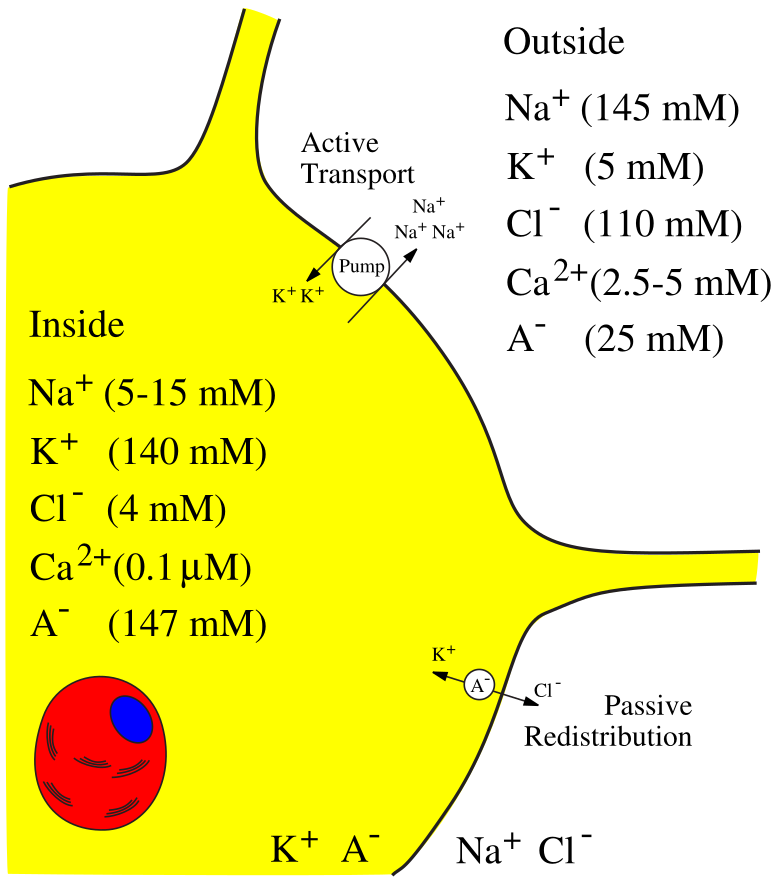
\includegraphics[height=1.4\textheight]{./neuron_diagram.png}
\end{center}
\end{frame}

\begin{frame}[label={sec:org9d26e4a}]{Whistlestop tour of electrophysiology}
\framesubtitle{Slow-fast spiking}

The interplay of slow potassium and fast sodium currents causes neurons to spike, rather than settling to a steady state

\begin{itemize}[<+->]
\item Sodium currents switch on and off fast
\item Potassium currents switch on and off slowly
\item Slow potassium activation allows the membrane potential to increase fast
\item Once it activates, the potassium current pulls the membrane potential back down
\item Potassium current takes a while to switch off again, so membrane potential gets pulled down to below the turn-on threshold for the two currents
\end{itemize}
\end{frame}


\begin{frame}[label={sec:orga71ab97}]{Whistlestop tour of electrophysiology}
\framesubtitle{Hodgkin-Huxley formalism}

\begin{columns}
\begin{column}{0.5\columnwidth}
Currents flow through different ion channels; let's consider each one separately.
Using current laws,

\begin{equation}
    C\dot{V} = I_{Na} + I_{Ca} + I_{K} + I_{Cl}~.
\end{equation}

The Hodgkin-Huxley model gives each ionic current as a function of membrane potential.
This is exciting, as we now have a mathematical model of a neuron, to which we can apply a rigorous analysis.
\end{column}

\begin{column}{0.5\columnwidth}
\begin{center}
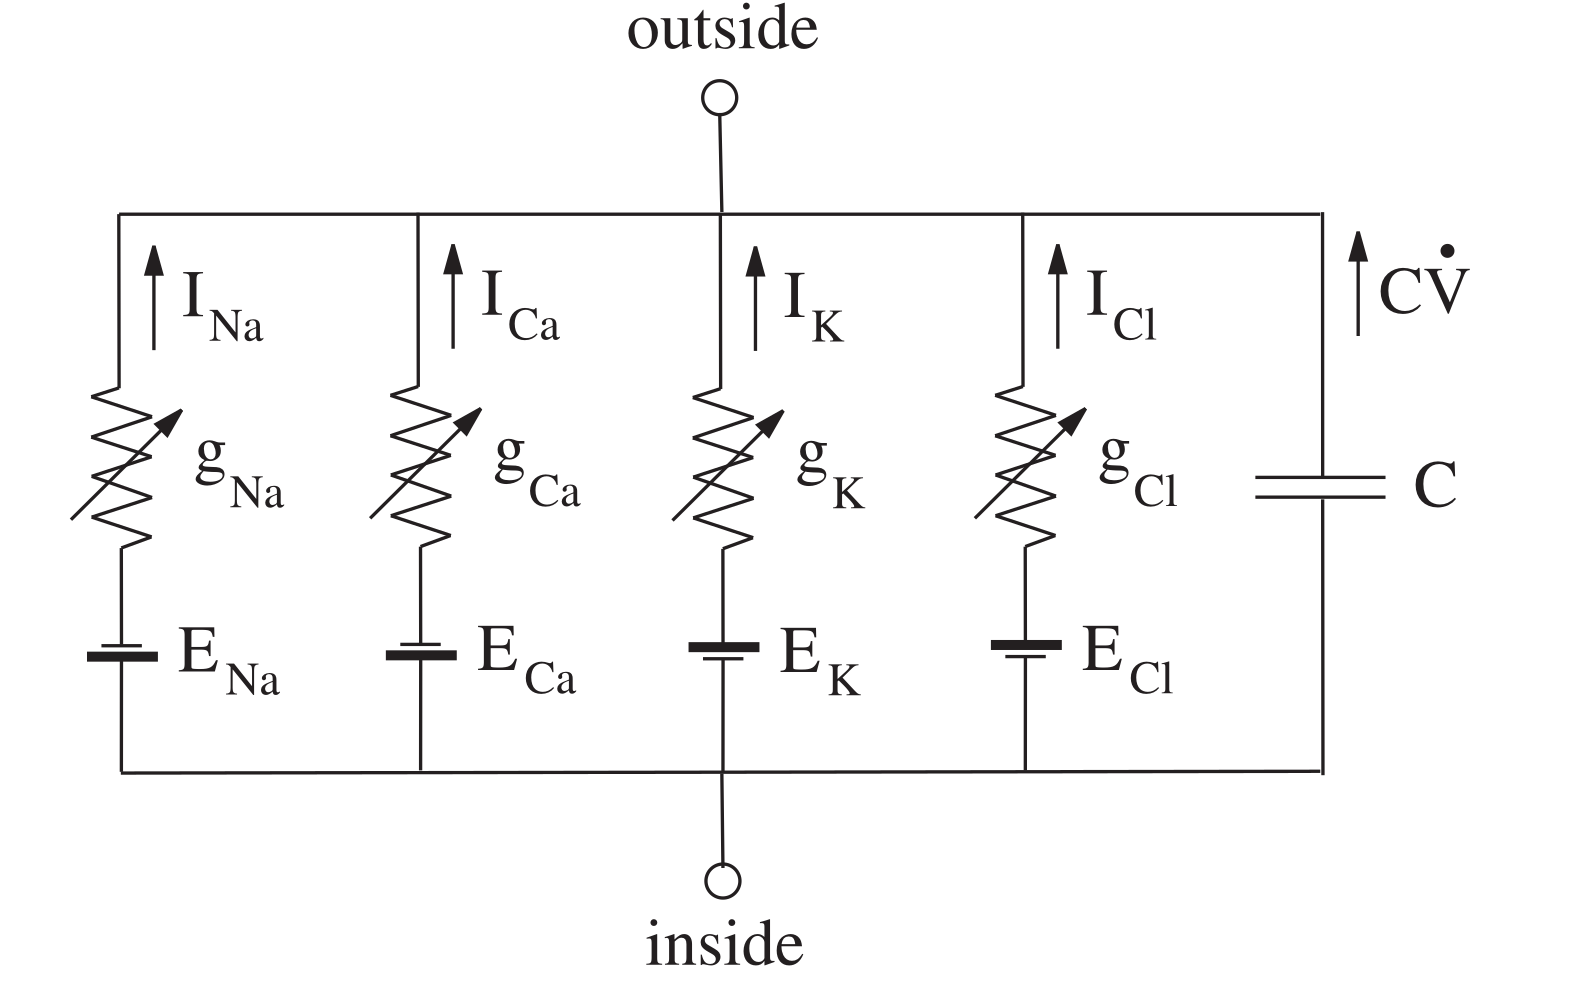
\includegraphics[width=.9\linewidth]{./neuroncircuit.png}
\end{center}
\end{column}
\end{columns}
\end{frame}


\begin{frame}[label={sec:org61c3a39}]{Presentation plan}
\begin{itemize}
    \item How do neurons work?
    \item \alert{Why should mathematicians get excited by neurons?}
\item What is my research topic? Why am I doing what I'm doing?
\item What challenges am I trying to solve, and how?
\end{itemize}
\end{frame}

\begin{frame}[label={sec:org2c662e7}]{Why are mathematicians interested in neurons?}
Neurons exhibit a wide range of complex dynamics.
Mathematical models of these dynamics can be easily tested on physical neurons.
Interesting features include\ldots{}
\begin{itemize}[<+->]
\item All neuron models are highly nonlinear
\item Biophysically accurate models are high-dimensional
\item The dynamics operate over multiple timescale dynamics
\item Neurons are a stochastic system
\item The Hogkin-Huxley model has a chaotic threshold set
\end{itemize}
\end{frame}


\begin{frame}[label={sec:org61c3a39}]{Presentation plan}
\begin{itemize}
    \item How do neurons work?
    \item Why should mathematicians get excited by neurons?
    \item \alert{What is my research topic? Why am I doing what I'm doing?}
\item What challenges am I trying to solve, and how?
\end{itemize}
\end{frame}

\begin{frame}{Project goal}
  \begin{itemize}[<+->]
    \item All results from neuroscience can be explained in terms of dynamical systems theory
    \item The current approach is to use numerical continuation to study bifurcations in models of neurons
    \item My goal: develop a control-based continuation method, to produce a model-free analysis of neuron bifurcations, on living cells
  \end{itemize}
\end{frame}

\begin{frame}[plain]
\begin{center}
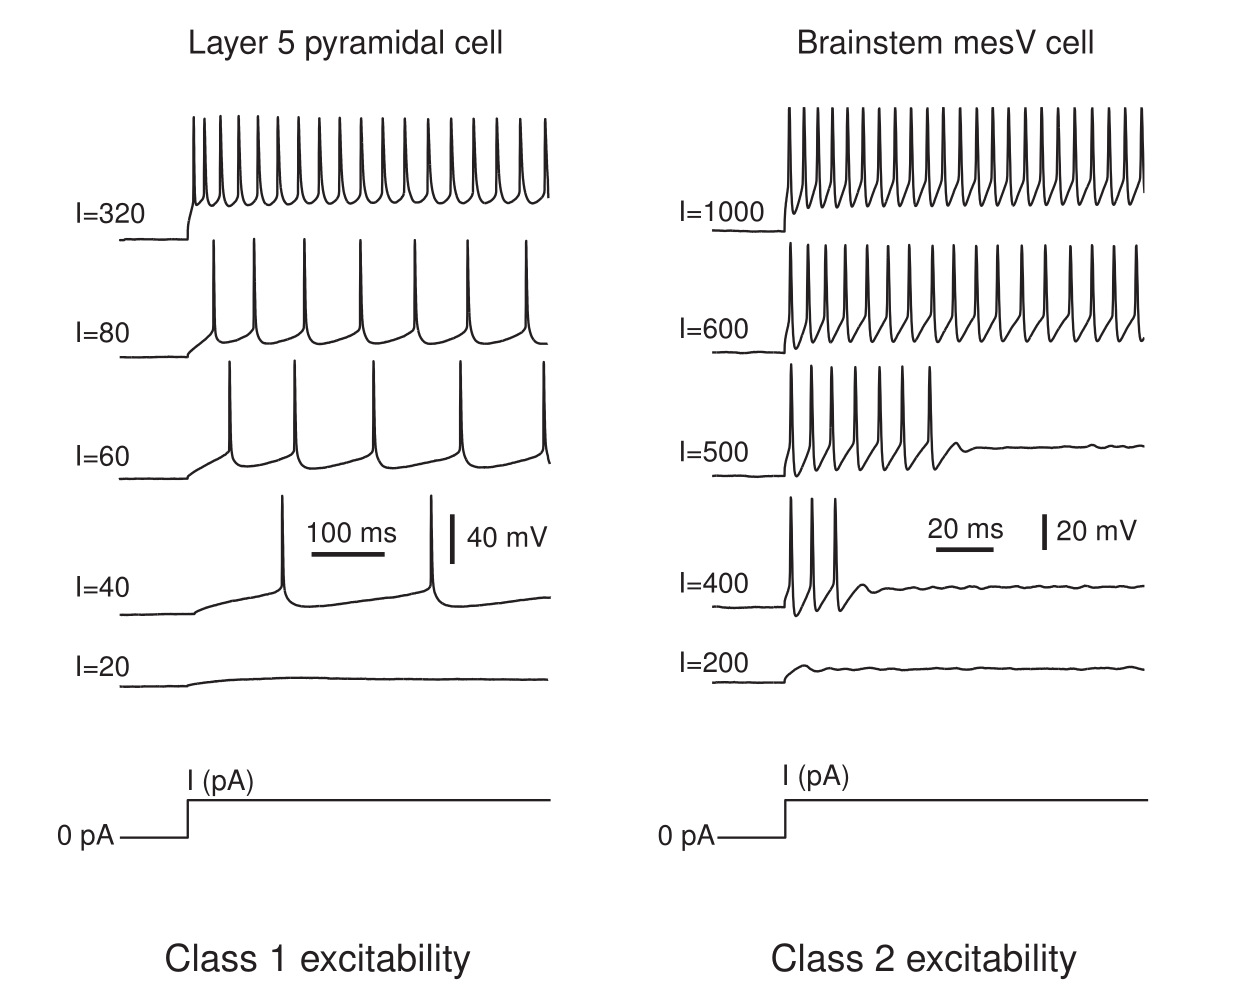
\includegraphics[height=1.4\textheight]{./excitability_classes.png}
\end{center}

\end{frame}
\begin{frame}[plain]
\begin{center}
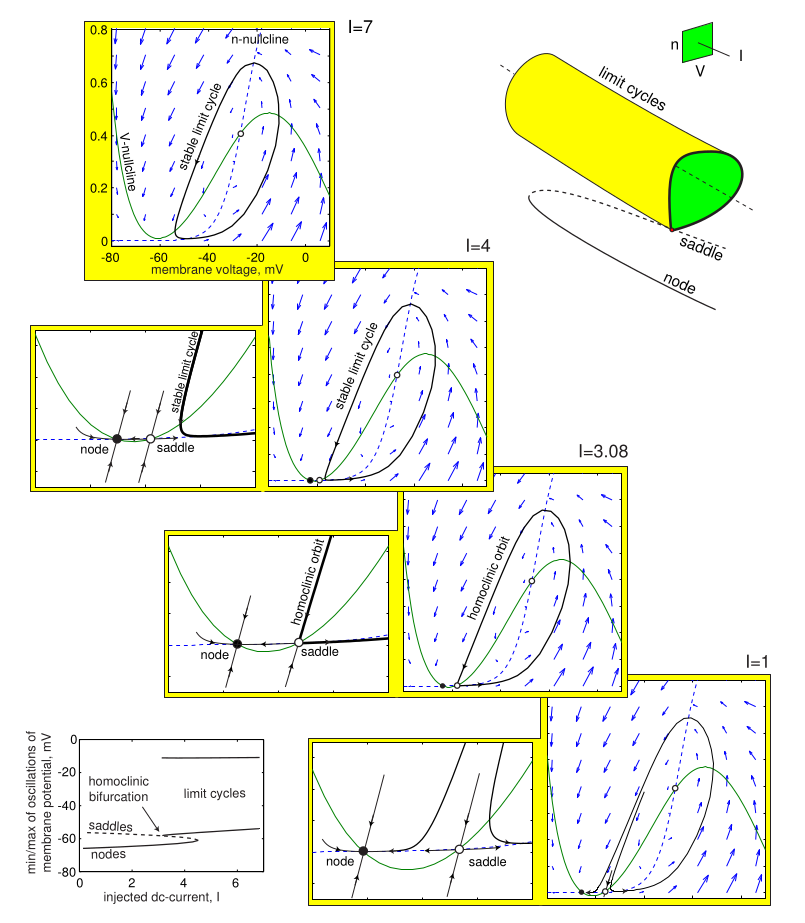
\includegraphics[height=1.4\textheight]{./homoclinic.png}
\end{center}
\end{frame}



\begin{frame}[label={sec:orgdead0e3}]{Project goal}
Goal: develop a method of observing bifurcations in the dynamics of living neurons.


\vspace{1cm}
\begin{block}{George Box}
All models are wrong, but some are useful
\end{block}
\end{frame}


\begin{frame}[label={sec:orgb87e419}]{Numerical continuation}
Consider \(f(x,\lambda)=0\).
Numerical continuation seeks to track \(x\), as \(\lambda\) varies.
For ODEs of form

$$\dot{x} = f(x,\lambda)~~,$$

this can be used to find bifurcations.
\end{frame}


\begin{frame}[label={sec:org3c374c7}]{Control-based continuation}
CBC allows us to apply continuation methods on black-box numerical or physical systems, no model needed.

\begin{itemize}
\item Use control theory to steer the system onto a (possibly unstable) natural invariant set
\item Track that invariant set as the bifurcation parameter changes
\end{itemize}

This tracking step can be a classical psuedo-arclength continuation, or something more problem-specific.
\end{frame}



\begin{frame}[label={sec:org61c3a39}]{Presentation plan}
\begin{itemize}
    \item How do neurons work?
    \item Why should mathematicians get excited by neurons?
    \item What is my research topic? Why am I doing what I'm doing?
    \item \alert{ What challenges am I trying to solve, and how?}
\end{itemize}
\end{frame}


\begin{frame}[label={sec:org8274cc8}]{Research problems}
\begin{itemize}[<+->]
\item Neurons are inherently stochastic; how do we deal with controlling and analysing this?
\item The system has poor observability (eg. can't easily see population ion channel conductance); how do we control a system that we can't observe?
\item We have limited control inputs; how can we use them to steer the dynamics effectively?
\item How do we control a highly nonlinear black-box system?
\item How can CBC be extended to study global bifurcations?
\end{itemize}
\end{frame}
\end{document}
